
% Prepared by Calvin Kent
%
% Assignment Template v19.02
%
%%% 20xx0x/MATHxxx/Crowdmark/Ax
%
\documentclass[12pt]{article} %
\usepackage{amsthm}
\usepackage{CKpreamble}
\usepackage{CKassignment}
\usepackage{mdframed}
\usepackage{import}
\usepackage{pdfpages}
\usepackage{transparent}
\usepackage{xcolor}
\usepackage{tkz-euclide}
\usepackage{physunits}
\usepackage{physics}
\usepackage{lmodern}
\usepackage{microtype}
\usepackage{upgreek}
\usepackage[misc]{ifsym}

%%% Maths and science packages

\usepackage{amsmath,amsthm,amssymb}
\usepackage{pgfplots}
	\usetikzlibrary{
		calc,
		patterns,
		positioning
	}
	\pgfplotsset{
		compat=1.16,
		samples=200,
		clip=false,
		my axis style/.style={
			axis x line=middle,
			axis y line=middle,
			legend pos=outer north east,
			axis line style={
				->,
			},
			legend style={
				font=\footnotesize
			},
			label style={
				font=\footnotesize
			},
			tick label style={
				font=\footnotesize
			},
			xlabel style={
				at={
					(ticklabel* cs:1)
				},
				anchor=west,
				font=\footnotesize,
			},
			ylabel style={
				at={
					(ticklabel* cs:1)
				},
				anchor=west,
				font=\footnotesize,
			},
			xlabel= $x$,
			ylabel=$\vec d (\m \tx{[East]})$
		},
	}
	\tikzset{
		>=stealth
	}

%%% Tables and figures packages

\usepackage{float}
\usepackage{caption}
	\captionsetup{
		format=plain,
		labelfont=bf,
		font=small,
		justification=centering
	}

\newcommand{\incfig}[2][1]{%
    \def\svgwidth{#1\columnwidth}
    \import{./figures/}{#2.pdf_tex}
}

\pdfsuppresswarningpagegroup=1


%
\begin{document}
	\pagenumbering{arabic}
	% Start of class settings ...
	\renewcommand*{\coursecode}{MATH 235} % renew course code
	\renewcommand*{\assgnnumber}{Assignment 1} % renew assignment number
	\renewcommand*{\submdate}{September 14, 2021} % renew the date
	\renewcommand*{\studentfname}{Abdullah} % Student first name
	\renewcommand*{\studentlname}{Zubair} % Student last name
    \renewcommand*{\proofname}{Proof:}
	% \renewcommand*{\studentnum}{20836288} % Student number

	\renewcommand\qedsymbol{$\blacksquare$}
	\setfigpath
	% End of class settings	
	% \pagestyle{crowdmark}
	\newgeometry{left=18mm, right=18mm, top=22mm, bottom=22mm} % page is set to default values
	\fancyhfoffset[L,O]{0pt} % header orientation fixed
	% End of class settings
	%%% Note to user:
	% CTRL + F <CHANGE ME:> (without the angular brackets) in CKpreamble to specify graphics paths accordingly.
	% The command \circled[]{} accepts one optional and one mandatory argument.
	% Optional argument is for the size of the circle and mandatory argument is for its contents.
	% \circled{A} produces circled A, with size drawn for letter A. \circled[TT]{A} produces circled A with size drawn for TT.
	% https://github.com/CalvinKent/My-LaTeX
	%%%

	%%%%%%%%%%%%%%%%%%%%%%%%%%%%%%%%%%%%%%%%%%%%%%%%%%%%%%%%%%%%%%%%%%%%%%%%%%%%%%%
	%%%                        CUSTOM MACRO VIM-TEX                             %%%
	%%       call IMAP('NOM', '\nomenclature{}', 'tex')               

	%%%%%%%%%%%%%%%%%%%%%%%%%%%%%%%%%%%%%%%%%%%%%%%%%%%%%%%%%%%%%%%%%%%%%%%%%%%%%%%

	% Crowdmark assignment start
	% qnumber, qname, qpoints

\begin{center}
	\textbf{\underline{\Huge{Solutions Test 1 - Review}}}
\end{center}
\begin{qstn} Solution:
  (Check with me)
\end{qstn}

\begin{qstn} Solution:
  \begin{enumerate}[label=(\alph*)]
    \item $H = \{4,5,6,7,8,\cdots\} $.
    \item $R = \{-1,0,1,2,3,4\} $.
    \item $A = \{2,-2\} $.
  \end{enumerate}
\end{qstn}

\begin{qstn} Solution:
\begin{center}
 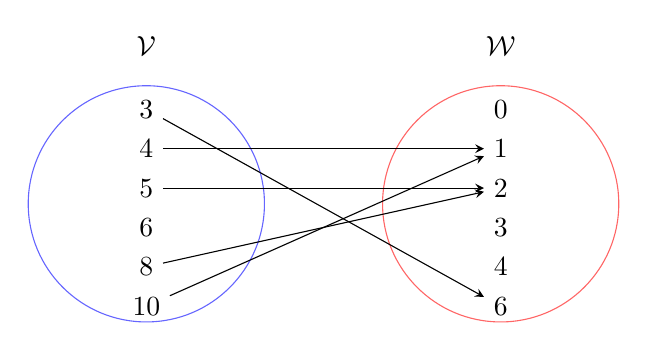
\begin{tikzpicture}
    % draw the sets
    \filldraw[fill=white!20, draw=blue!60] (-1.5,0) circle (1.5cm);
    \filldraw[fill=white!20, draw=red!60] (3,0) circle (1.5cm);


    % the texts
    \node at (-1.5,2) {$\mathcal{V}$};
    \node at (3,2) {$\mathcal{W}$};

    % the points in the sets (here I just create nodes to use them later on to position
    % the circles and the arrows
    \node (x1) at (-1.5,1.2) {$3$};
    \node (x2) at (-1.5,0.7) {$4$};
    \node (x3) at (-1.5,0.2) {$5$};
    \node (x4) at (-1.5,-0.3) {$6$};
    \node (x5) at (-1.5,-0.8) {$8$};
    \node (x6) at (-1.5,-1.3) {$10$};
    \node (y1) at (3,1.2) {$0$};
    \node (y2) at (3,0.7) {$1$};
    \node (y3) at (3,0.2) {$2$};
    \node (y4) at (3,-0.3) {$3$};
    \node (y5) at (3,-0.8) {$4$};
    \node (y6) at (3,-1.3) {$6$};

     %draw the arrows
    \draw[->] (x1) -- (y6);

    \draw[->] (x2) -- (y2);

    \draw[->] (x3) -- (y3);

    \draw[->] (x5) -- (y3);

    \draw[->] (x6) -- (y2);

\end{tikzpicture}
\end{center}
\end{qstn}


\begin{qstn} Solution:
  \begin{enumerate}[label=(\alph*)]
    \item $T(T(1)) = 175$.
    \item $H(H(-2)) = -4$.
    \item $T(H(0)) = -1$. 
    \item $T(x) = x(3x + 4)$.
    \item 
       \begin{align*}
         T(H(x)) &= 3\left( x-1 \right) ^2 + 4\left( x - 1 \right) \\
                 &= 3(x^2 - 2x + 1) + 4(x-1)\\
                 &= 3x^2 - 6x + 3 + 4x - 4\\
                 &= 3x^2 - 2x - 1
      .\end{align*}
      The two integers you should get are $p = 1, q = -3$. (How you label it is up to you), afterwards we need.
       \begin{itemize}
         \item $t = \gcd(\left|a\right|, \left|p\right|) = \gcd(\left|3\right|, \left|1\right|) = \gcd(3,1) = 1$.
         \item $k = \gcd(\left|q\right|, \left|c\right|) = \gcd(\left|-3\right|, \left|-1\right|) = \gcd(3,1) = 1$.
      \end{itemize}
      Since $a \cdot q = 3 \cdot -3 = -9 $, we conclude that $a \cdot q < 0$ and hence,
      \[
            T(H(x)) = (tx - k)\left( \frac{a}{t}x + \frac{p}{t} \right) = (x - 1)(3x + 1)
      .\] 
  \end{enumerate}
\end{qstn}

\newpage

\begin{qstn}
  Solution:
  \begin{enumerate}[label=(\alph*)]
    \item $\mathcal{D} = \{x\in \R \mid x \leq 2\} $, $\mathcal{R} = \{y \in \R \mid y \leq -7\}$.
    \item $\mathcal{D} = \R $, $\mathcal{R} = \{y \in \R \mid y \leq 6\}$.
    \item $\mathcal{D} = \R $, $\mathcal{R} = \R$.
    \item $\mathcal{D} = \R $, $\mathcal{R} = \{ y\in \R \mid y \geq -5\} $.
    \item $\mathcal{D} = \{x\in \R \mid x \neq \frac{2}{5}\}  $, $\mathcal{R} = \{ y\in \R \mid y \geq 4\} $.
    \item $\mathcal{D} = \{x\in \R \mid -3 \leq x \leq 1\}  $, $\mathcal{R} = \{ y\in \R \mid -2 \leq y \leq 2\} $.
  \end{enumerate}
\end{qstn}



\begin{qstn}
  Solution:
  \begin{enumerate}[label=(\alph*)]
    \item By the discriminant formula we have,
      \begin{align*}
        d &= b^2 - 4ac\\
          &= (5)^2 - 4(2)(-3)\\
          &= 25 + 24\\
          &= 49
      .\end{align*}
      Because $d > 0$ we conclude that $f(x)$ will have two \textbf{distinct} solutions.

    \item 
      The two integers you should get are $p = -1, q = 6$. (How you label it is up to you), afterwards we need.
       \begin{itemize}
         \item $t = \gcd(\left|a\right|, \left|p\right|) = \gcd(\left|2\right|, \left|-1\right|) = \gcd(2,1) = 1$.
         \item $k = \gcd(\left|q\right|, \left|c\right|) = \gcd(\left|6\right|, \left|-3\right|) = \gcd(6,3) = 3$.
      \end{itemize}
      Since $a \cdot q = 2\cdot 6 = 12 $, we conclude that $a \cdot q > 0$ and hence,
      \[
            f(x) = (tx + k)\left( \frac{a}{t}x + \frac{p}{t} \right) = (x + 3)(2x - 1)
      .\] 

    \item How you label them is up to you,
      \[
            x_1 = -3, \,\,\,\, x_2 = \frac{1}{2}
      .\] 
    \item From part (c) we have the x-intercepts so we can skip step 1. Proceeding with calculating $h$,
      \[
          h = \frac{x_1 + x_2}{2} = \frac{-3 + \frac{1}{2}}{2} =  -\frac{5}{4}
      .\] Now $k$,
      \begin{align*}
        k &= f(h)\\
          &= f(-\frac{5}{4})\\
          &= 2\left( -\frac{5}{4} \right) ^2 + 5\left( -\frac{5}{4} \right) - 3\\
          &= \frac{50}{16} - \frac{25}{4} - 3 = -\frac{98}{16}
      .\end{align*}

      Lastly $a$,
      \[
        a = b \cdot m \cdot k = 1 \cdot  1 \cdot  2 = 2
      .\] 
      Finally we have $f(x)$ in vertex form,
       \[
          f(x) = 2\left( x + \frac{5}{4} \right) ^2 - \frac{98}{16}
      .\] 
    \item 
      Solution:
    \begin{center}
        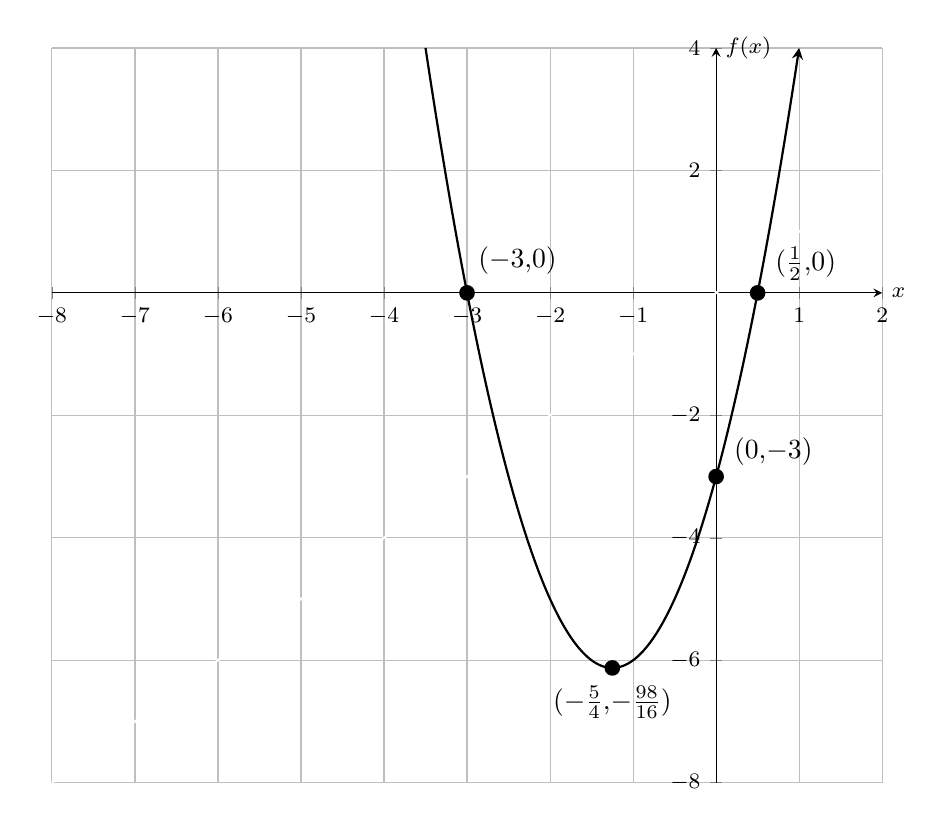
\begin{tikzpicture}
        \begin{axis}[
            my axis style,
            width=\textwidth,
            height=0.9\textwidth,
            ylabel=$f(x)$,
            grid
        ]
        
        \addplot[
            domain=-8:2,
            thick,
            white,
            -
        ]
        {x};

        \addplot[
            domain=-3.5:1,
            thick,
            black,
            ->
        ]
        {2*(x+1.25)^2-6.125};

        \fill[
            black
        ];


        \node[label={80:{($-3$,$0$)}},circle,fill,inner sep=2pt] at (axis cs:-3,0) {};
        \node[label={19:{($\frac{1}{2}$,$0$)}},circle,fill,inner sep=2pt] at (axis cs:0.5,0) {};
        \node[label={10:{($0$,$-3$)}},circle,fill,inner sep=2pt] at (axis cs:0,-3) {};
        \node[label={270:{($-\frac{5}{4}$,$-\frac{98}{16}$)}},circle,fill,inner sep=2pt] at (axis cs:-1.25,-6.125) {};

     

        \end{axis}
        \end{tikzpicture}
    \end{center}

  \end{enumerate}
\end{qstn}
































\end{document}




















